\Chapter{MÉTHODOLOGIE}\label{sec:Methodologie}


La section méthodologique sera divisée en trois sections. La première présentera les jeux de données disponibles dans le contexte de la ville de Québec. La deuxième présentera une plan d'ensemble de la méthodologie et des moyens encourus pour faire l'inventaire du stationnement et la troisième.


\section{Données}
  Le tableau \ref{tab:donnees_disponibles_Québec} résume les données disponibles pour la ville de Québec et leur source.
  \begin{landscape}
    \LTcapwidth=\textwidth
  \begin{longtable}[h!]{p{.2 \linewidth} p{.1 \linewidth} p{.3 \linewidth} p{.15\linewidth} p{.125\linewidth} }
    
    
    \hline
    Géobase & Type & Description  & Source & Date téléchargement.\\ 
    \hline
    \hline
    \endhead
    \hline
    \endfoot
    \hline
    \caption{Géobases pour le territoire de la ville de Québec}
    \label{tab:donnees_disponibles_Québec}
    \endlastfoot
    
    
    vdq-panneaux stationnement    & Points        & Panneaux de stationnement sur rue          & Ville de Québec / Données Québec  & 5 mai 2024 \\
    \hline
    vq\_quartiers & Polygones & SIG des quartiers de la ville de Québec & Ville de Québec / Données Québec & 5 mai 2024 \\
    \hline
    vdq-bornesfontaines          & Points        & Bornes fontaines sur rue                   & Ville de Québec / Données Québec & 12 mai 2024 \\
    \hline
    vq\_reseau\_routier\_2023 & Polylignes    & Bords de voiries pour circulation automobile  & Ville de Québec / Geo-index  & 12 juin 2023\\ 
    \hline
    vq\_stationnement\_2021  & Polylignes    & Bords des aires de stationnement hors rue & Ville de Québec / Geo-index & 8 mai 2021\\
    \hline
    vdq\_voie\_publique            & Lignes        & Centres de chaussées trottoirs séparés et pistes cyclables & Ville de Québec / Données Québec & 16 avril 2024 \\
    \hline
    vdq-zonage-grille.xlsx          & Tableau        & Usages autorisés et classification (urbain/structurant/général) & Ville de Québec / Données Québec & 8 juin 2024 \\
    \hline
    vdq-zonagemunicipalzones          & Polygones        & Unités de voisinages selon le zonage municipal & Ville de Québec / Données Québec & 6 mai 2024 \\
    \hline
    vdq\_intersection\_voie \_publique & Points & Intersections avec les dispositifs de contrôle & Ville de Québec / Données Québec & 8 mai 2024 \\
    \hline
    vdq\_quartiers & Polygones &Séparation de la ville en quartiers & Ville de Québec / Données Québec & 8 mai 2024\\
    \hline
    Usages prédominants 2023  & Polygones & Usages prédominants du sol &   Ministère des Affaires municipales et de l'Habitation & 21 mai 2024 \\
    \hline
    Arrêts bus et à vélo 2024 & Points et polylignes & Arrêts de bus, parcours des lignes et bornes vélo-partage & Réseau de transport de la capitale & 31 mai 2023 \\
    \hline
    Année de construction des chaussées & Polylignes & Année de construction des rues & Ville de Québec / Géoindex & 28 mai 2024 \\
    \hline
    Rôle foncier & Entrées de tableaux & Données en format xml du rôle foncier & Ministère des Affaires municipales et de l'Habitation & 28 mai 2024 \\
    \hline
    Rôle foncier géobase & FGDB (Points + tables) & Données SIG du rôle foncier & Ministère des Affaires municipales et de l'Habitation & 28 mai 2024 \\
    \hline
    highway & Polylignes & Centres de chaussées & \ac{OSM} & 13 mai 2024\\
    \hline
    parking & points et polygones & Stationnement recensés dans \ac{OSM} & \ac{OSM} & 2 mai 2024 \\
    \hline
      parking entrance & Points & Entrées de stationnement sous-terrains  & \ac{OSM} & 2 mai 2024 \\
      \hline
    
  \end{longtable}

  \begin{table}[h!]
    \centering
    \begin{tabular}{p{0.18\linewidth} | p{0.1\linewidth} | p{0.3\linewidth} | p{0.3\linewidth}} 
    \hline
    Nom du champs & Type Contenu & Description  & Exemple\\ 
    \hline
    ID             & Entier    & Entier identifiant unique pour chaque panneau  & 370758 \\ 
    & & & \\
    TYPE\_CODE      & Texte     & Code d'identification de chaque type de panneau de stationnement & PP1016\\
    & & & \\
    DESCRIPTION     & Texte     & Texte imprimé sur le panneau & Stat. int. 16h-18h LUN À VEN (fl. dou.)\\
    \hline
    \end{tabular}
    \caption{Champs de la géobase de panneaux de stationnement de la ville de Québec \parencite{VilledeQuebec:PanneauxSignalisation:2024}}
    \label{tab:champs_geobase_stationnement_quebec}
  \end{table}
  \end{landscape}
\section{Illustration des données acquises}
  La section suivante va donner un aperçu de quelques intersections typiques pour illustrer les données disponibles. Les mêmes quelque cas seront illustrés à des fins illustratives. Le but principal est d'illustrer les enjeux.
    \subsection{Illustration - Cas 1: Coin Gomin / Marguerite-Bourgeoys / Laurier}
      Les figures \ref{fig:donnes_panneaux_Laurier} et \ref{fig:donnes_polygone_panneaux_Laurier} donnent un aperçu des données disponibles pour l'intersection nommée ci-dessus. On constate que plusieurs panneaux sur un même poteau ne sont pas représentés géographiquement au même endroit. D'autre part, la présence de panonceaux donne des exceptions aux limitations de temsp de stationnement. De plus, la ville a à sa disposition une géobase de bords de rue mais aucune information n'est disponible pour associer le bord de rue à un tronçon donné. Le même constat est possible pour les panneaux de stationnement dont les seuls informations sont un identifiant, la description et un identifiant de panneau. Ils ne sont pas associés à un tronçon ou un côté de rue. L'une des conséquences de la dispersion des panneaux est aussi la difficulté d'assigner les panneaux à un tronçon aux intersections puisque le panneau peut être plus proche d'un bord de rue autre du fait du décalage des panneaux dans l'espace. Dans ce cas-ci, le panneau Stat. int. (fl. ga.) est à 6m de la rue Marguerite Bourgeoys et 9m de la rue Gomin.
      \begin{figure}[ht]
        \centering
        \begin{subfigure}{\linewidth}
          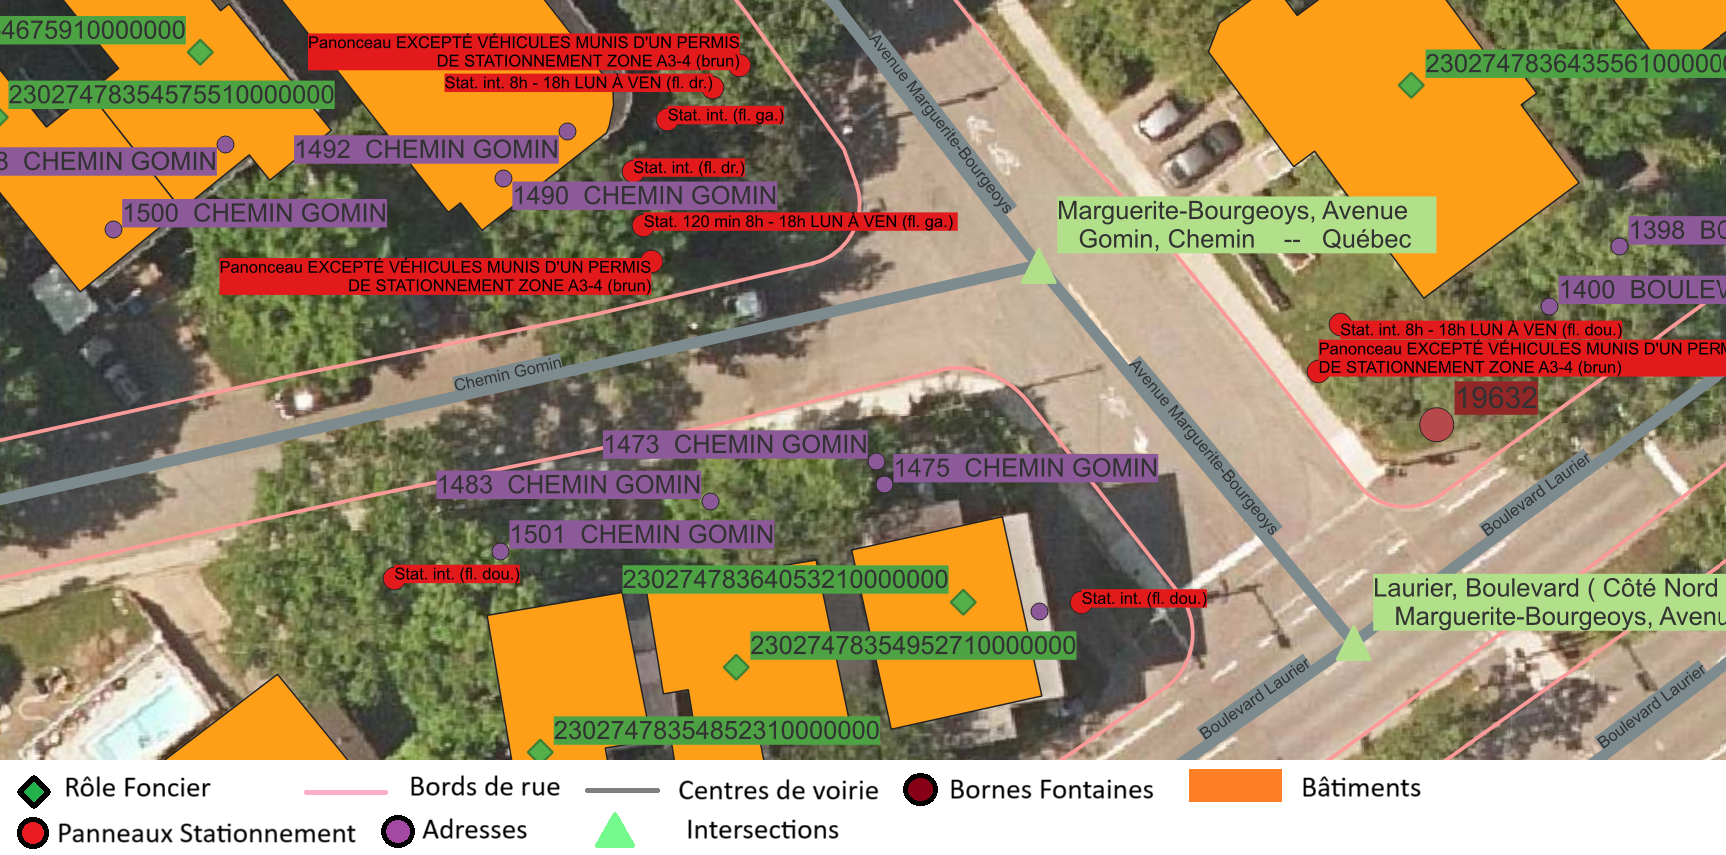
\includegraphics[width=1.0\textwidth]{images/donnees_disponible_Laurier_legende_v2.png}
        \caption{Données linéaires disponibles}
        \label{fig:donnes_panneaux_Laurier}
        \end{subfigure} \\
        \begin{subfigure}{\linewidth}
          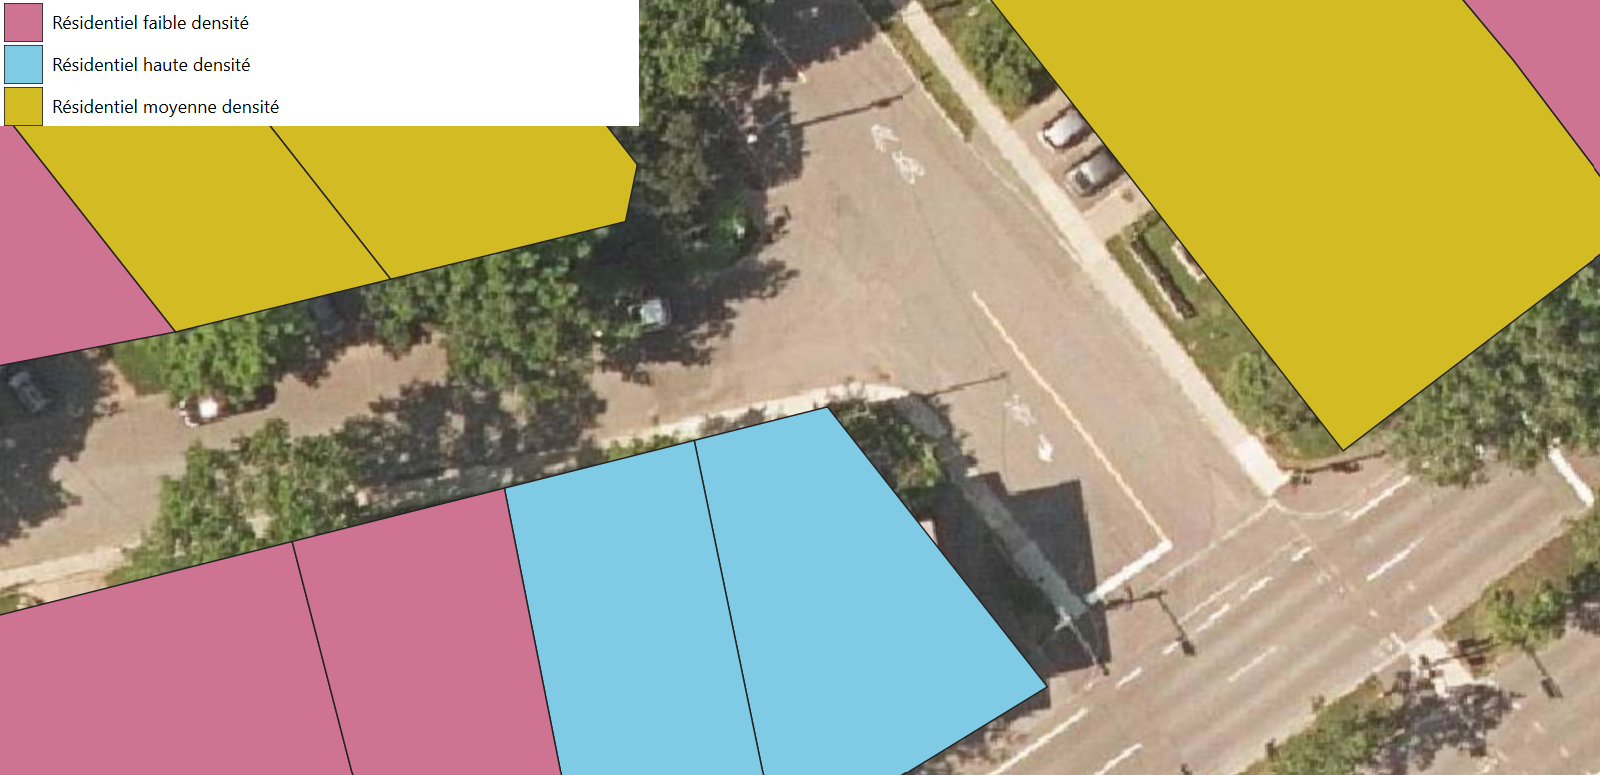
\includegraphics[width=1.0\textwidth]{images/utilisation_sols_Laurier_v2.png}
        \caption{Données polygonales disponibles}
        \label{fig:donnes_polygone_panneaux_Laurier}
        \end{subfigure}
        \caption{Données disponicles intersection Laurier}
      \end{figure}

      \FloatBarrier
  \subsection{Illustration - Cas 2: Coin de la Canardières - Desroches}
  Les figures \ref{fig:donnes_panneaux_Desroches} et \ref{fig:donnes_polygone_panneaux_Desroches} illustre les mêmes données à un autre coin de rue. Ici, la localisation des panneaux porte encore plus à confusion puisque les panneaux de 2 tronçons de rue sont quasiment superposés. Il sera donc difficile d'assigner les panneaux aux bords de rues automatiquement lorsque ces derniers sont aux abords des intersections.
  \begin{figure}[ht]
    \centering
    \begin{subfigure}{\linewidth}
      \centering
      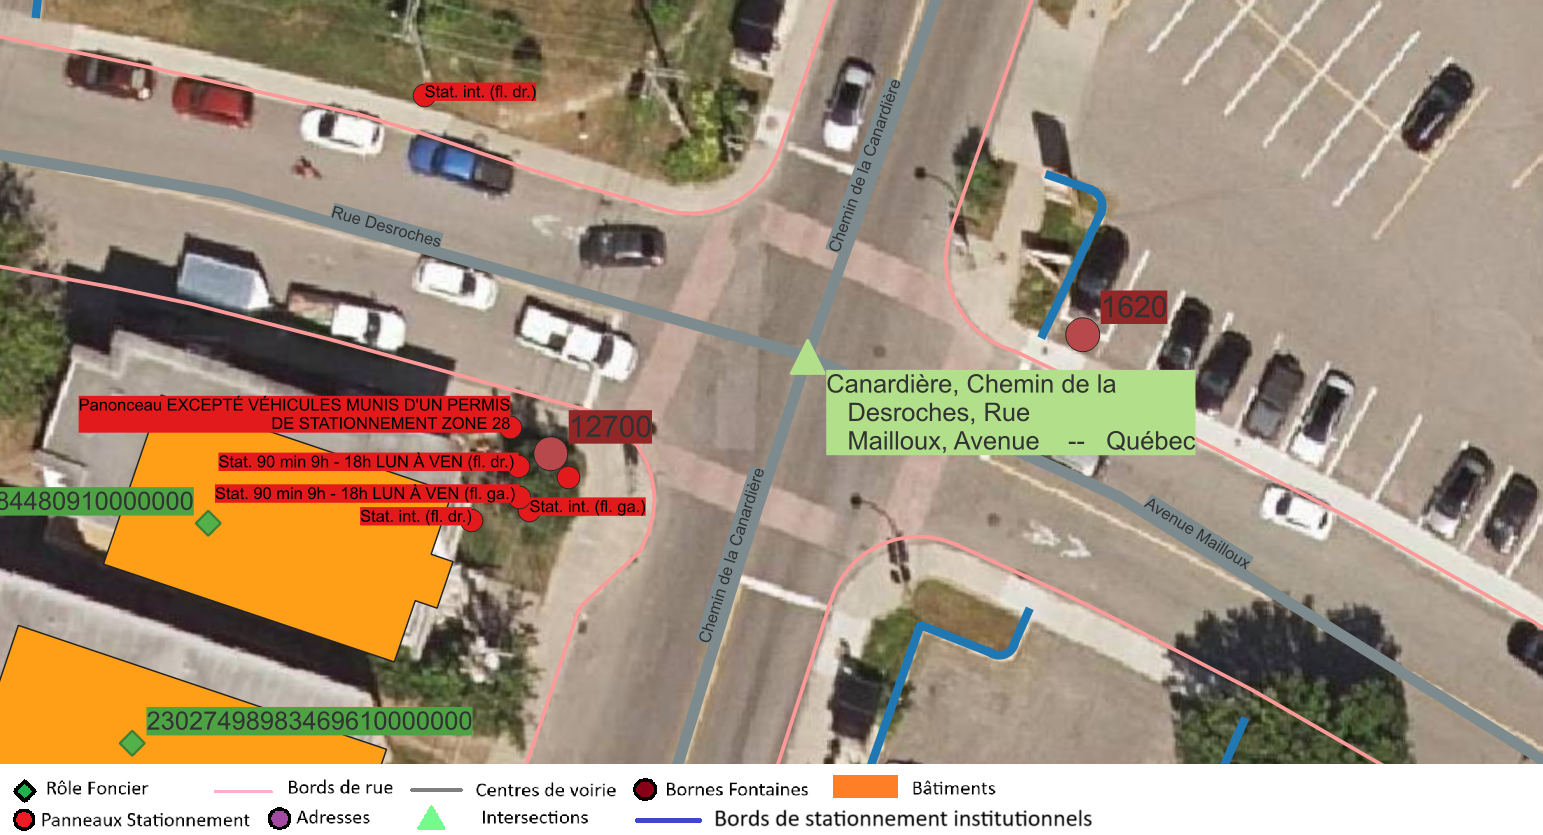
\includegraphics[width=0.8\textwidth]{images/donnees_disponible_Desroches_legende_v2.png}
    \caption{Données linéaires disponibles}
    \label{fig:donnes_panneaux_Desroches}
    \end{subfigure} \\
    \begin{subfigure}{\linewidth}
      \centering
      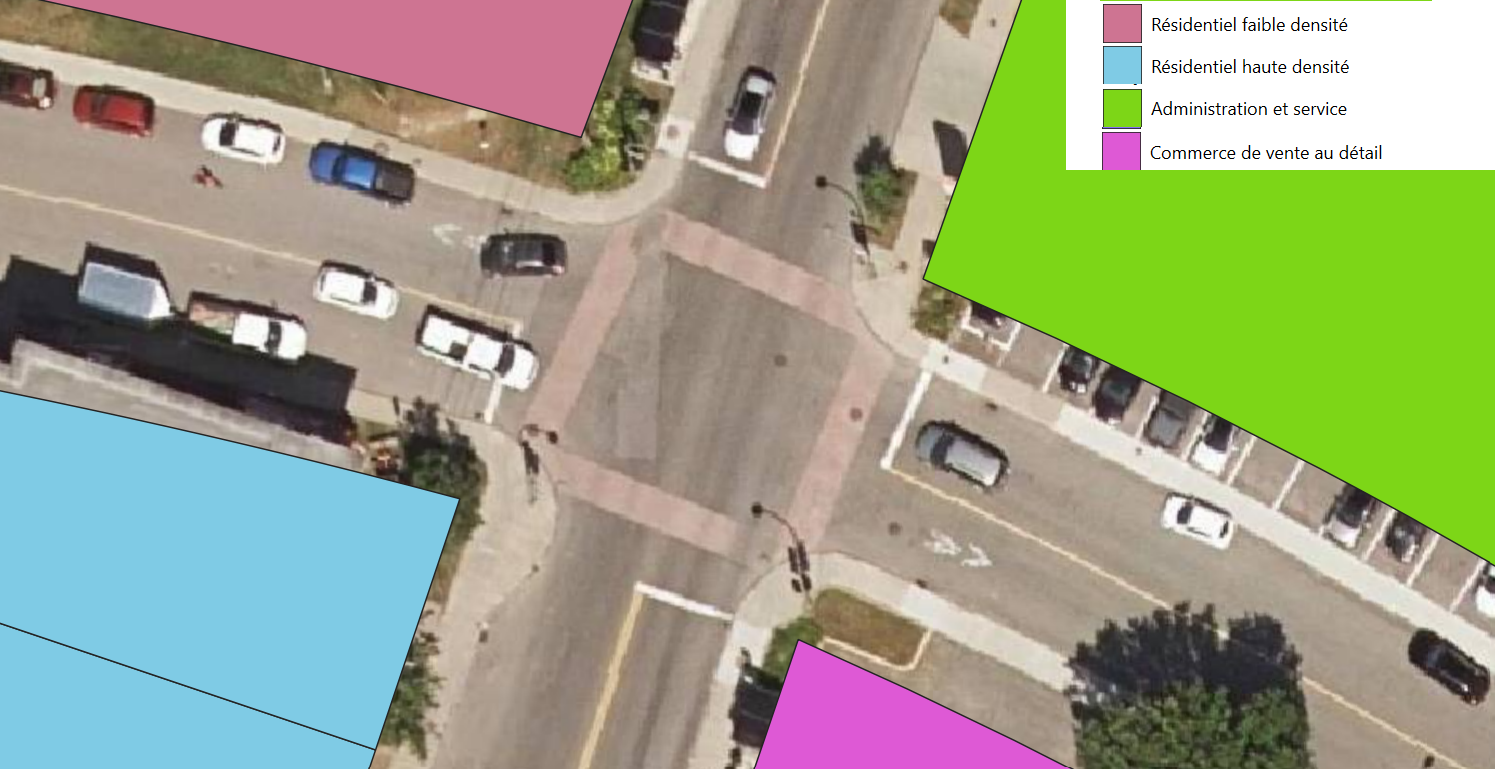
\includegraphics[width=0.8\textwidth]{images/utilisation_sols_Desroches_v2.png}
    \caption{Données polygonales disponibles}
    \label{fig:donnes_polygone_panneaux_Desroches}
    \end{subfigure}
    \caption{Données disponibles intersection Desroches / De la Canardière}
  \end{figure}
\FloatBarrier
\section{Données de panneaux de stationnement}
  Les panneaux ne sont pas classifiés de manière à être facilement lisible par machine. Aucun index des panneaux de stationnement n'existe à la connaissance de l'auteur. Une classification semi automatisée en isolant certains morceaux de chaînes de caractères a donc été crée pour rendre les panneaux de stationnement compatibles avec la structure de base de données énoncée dans \textcite{Bourdeau:MethodologieAnalyse:2014} et \textcite{Morency:DeveloppementMise:2022}. Le tableau \ref{tab:donnees_requises} liste les champs requis pour définir la fonction d'un panneau de stationnement:
  \LTcapwidth=\textwidth

  \begin{longtable}{p{0.15 \linewidth}  l p{0.5\linewidth} l  }
    \hline
    Champs & Type & Description & Valeur possibles \\
    \hline
    \endhead
    \hline
    \endfoot
    \hline
    \caption{Champs requis dans la base de données de stationnement}
    \label{tab:donnees_requises}
    \endlastfoot
    DUREE \_MAX\_ MINUTES & Entier & Durée maximale de stationnement & 0-120 \\
    TYPE\_1 & Entier & Clientèle spécifique de ce panneau & 0-11\\
    TYPE\_2 & Entier & Clientèle spécifique de ce panneau & 0-11\\
    ANNUEL & Booléen & Règlementation applicable à l'année & Vrai-Faux \\
    Date\_debut\_1 & Entier &  Date d'entrée en vigueur de la règlementation & 0-365\\
    Date\_fin\_1 & Entier & Date de fin de la règlementation & 0-365 \\
    Date\_debut\_2 & Entier & Date d'entrée en vigueur de la règlementation & 0-365 \\
    Date\_fin\_2 & Entier & Date de fin de la règlementation & 0-365 \\
    Q & Booléen & Règlementation applicable de manière quotidienne & Vrai - Faux \\
    Q\_d\_1 & Float & Heure d'entrée en vigueur de la règlementation & 0-24 \\
    Q\_f\_1 & Float & Heure de fin de la règlementation & 0-24\\
    Q\_d\_2 & Float & Heure de début de la deuxième période de validité de la règlementation 0-24\\
    LU & Booléen & Règlementation applicable un lundi (Q est nécessairement faux) & Vrai - Faux \\
    LU\_debut\_1 & Float & Heure d'entrée en vigueur de la règlementation & 0-24\\
    LU\_fin\_1 & Float & Heure d'arrêt de la règlementation & 0-24\\
    LU\_debut\_2 & Float & Deuxième Heure d'entrée en vigueur de la règlementation & 0-24\\
    LU\_fin\_2 & Float & Deuxième Heure d'arrêt de la règlementation & 0-24 \\
    MA & Booléen & Règlementation applicable un mardi (Q est nécessairement faux) & Vrai - Faux \\
    MA\_debut\_1 & Float & Heure d'entrée en vigueur de la règlementation & 0-24\\
    MA\_fin\_1 & Float & Heure d'arrêt de la règlementation & 0-24\\
    MA\_debut\_2 & Float & Deuxième Heure d'entrée en vigueur de la règlementation & 0-24\\
    MA\_fin\_2 & Float & Deuxième Heure d'arrêt de la règlementation & 0-24 \\
    ME & Booléen & Règlementation applicable un jeudi (Q est nécessairement faux) & Vrai - Faux \\
    ME\_debut\_1 & Float & Heure d'entrée en vigueur de la règlementation & 0-24\\
    ME\_fin\_1 & Float & Heure d'arrêt de la règlementation & 0-24\\
    ME\_debut\_2 & Float & Deuxième Heure d'entrée en vigueur de la règlementation & 0-24\\
    ME\_fin\_2 & Float & Deuxième Heure d'arrêt de la règlementation & 0-24 \\
    JE & Booléen & Règlementation applicable un jeudi (Q est nécessairement faux) & Vrai - Faux \\
    JE\_debut\_1 & Float & Heure d'entrée en vigueur de la règlementation & 0-24\\
    JE\_fin\_1 & Float & Heure d'arrêt de la règlementation & 0-24\\
    JE\_debut\_2 & Float & Deuxième Heure d'entrée en vigueur de la règlementation & 0-24\\
    JE\_fin\_2 & Float & Deuxième Heure d'arrêt de la règlementation & 0-24 \\
    VE & Booléen & Règlementation applicable un vendredi (Q est nécessairement faux) & Vrai - Faux\\
    VE\_debut\_1 & Float & Heure d'entrée en vigueur de la règlementation & 0-24\\
    VE\_fin\_1 & Float & Heure d'arrêt de la règlementation & 0-24\\
    VE\_debut\_2 & Float & Deuxième Heure d'entrée en vigueur de la règlementation & 0-24\\
    VE\_fin\_2 & Float & Deuxième Heure d'arrêt de la règlementation & 0-24 \\
    SA & Booléen & Règlementation applicable un samedi (Q est nécessairement faux) & Vrai - Faux \\
    SA\_debut\_1 & Float & Heure d'entrée en vigueur de la règlementation & 0-24\\
    SA\_fin\_1 & Float & Heure d'arrêt de la règlementation & 0-24\\
    SA\_debut\_2 & Float & Deuxième Heure d'entrée en vigueur de la règlementation & 0-24\\
    SA\_fin\_2 & Float & Deuxième Heure d'arrêt de la règlementation & 0-24 \\
    DI & Booléen & Règlementation applicable un samedi (Q est nécessairement faux) & Vrai - Faux \\
    DI\_debut\_1 & Float & Heure d'entrée en vigueur de la règlementation & 0-24\\
    DI\_fin\_1 & Float & Heure d'arrêt de la règlementation & 0-24\\
    DI\_debut\_2 & Float & Deuxième Heure d'entrée en vigueur de la règlementation & 0-24\\
    DI\_fin\_2 & Float & Deuxième Heure d'arrêt de la règlementation & 0-24 \\  
  \end{longtable}

  \FloatBarrier
\section{Règlementation de stationnement hors Rue}
  Le stationnement hors-rue est régi par le code d'urbanisme de la ville de Québec. Cette règlementation a été harmonisée en 2009 pour l'ensemble de la ville. Avant cela, les règles de différentes municipalités qui ont fusionnée ou scindé au cours des année ont régi la construction. À l'heure actuelle, quatre ensembles de règles de stationnement sont en places pour la ville de Québec:
  \begin{itemize}
    \item Urbain Dense 
    \item Axe Structurant A
    \item Axe Structurant B
    \item Générale
  \end{itemize}
  L'affectation a chacun de ces types est faite au niveau de l'unité de voisinage. La définition spatiale des unités de voisinage est donnée dans \textcite{VilledeQuebec:ZonageMunicipal:2024} et l'assignation de la zone est donnée dans \textcite{VilledeQuebec:GrilleSpecifications:2024}. La carte à la figure \ref{fig:types_unites_voisinage} montre les unités de voisinage pour la ville de Québec catégorisé selon la définition ci-haut:
  \begin{figure}
    \centering
    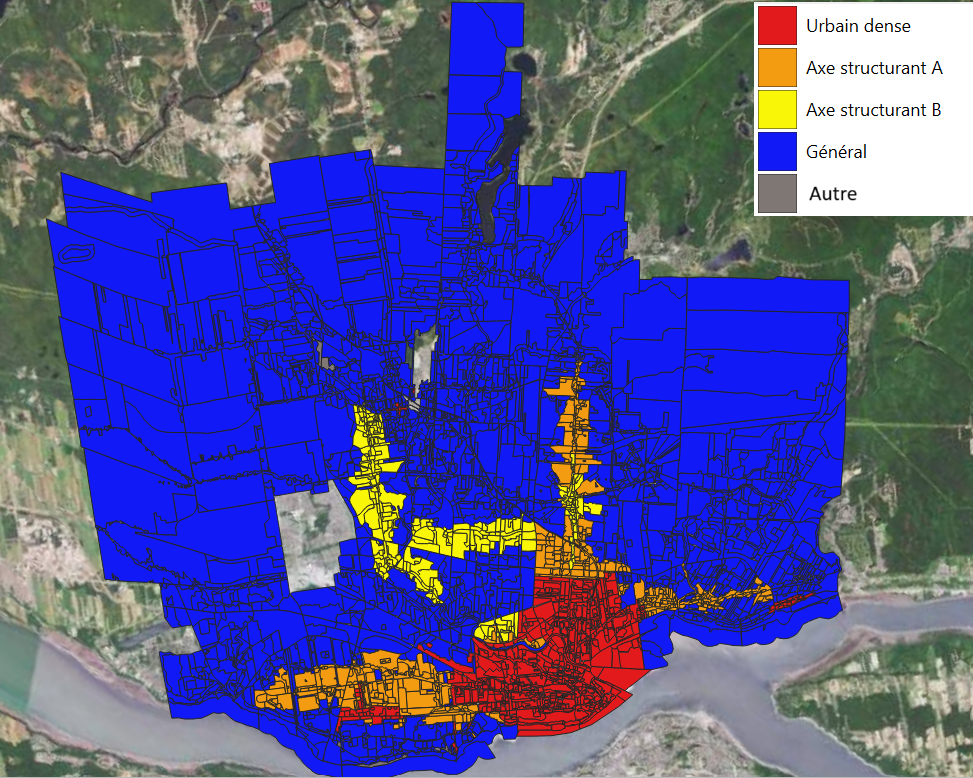
\includegraphics[width=0.5\linewidth]{images/Types_unites_voisinage.png}
    \caption{Types d'unités de voisinage}
    \label{fig:types_unites_voisinage}
  \end{figure}
  \FloatBarrier
\section{Données d'entrainement d'apprentissage machine}
Plusieurs ensembles de données ont été créés pour la détection de places ouvertes dans un stationnement. Plus récemment, un ensemble de données annotés a été créé pour 
